\documentclass{article}

% if you need to pass options to natbib, use, e.g.:
%     \PassOptionsToPackage{numbers, compress}{natbib}
% before loading neurips_2020

% ready for submission
% \usepackage{neurips_2020}

% to compile a preprint version, e.g., for submission to arXiv, add add the
% [preprint] option:
    \usepackage[preprint]{neurips_2020}

% to compile a camera-ready version, add the [final] option, e.g.:
%     \usepackage[final]{neurips_2020}

% to avoid loading the natbib package, add option nonatbib:
     \usepackage[nonatbib]{neurips_2020}

\usepackage[utf8]{inputenc} % allow utf-8 input
\usepackage[T1]{fontenc}    % use 8-bit T1 fonts
\usepackage{hyperref}       % hyperlinks
\usepackage{url}            % simple URL typesetting
\usepackage{booktabs}       % professional-quality tables
\usepackage{amsfonts}       % blackboard math symbols
\usepackage{nicefrac}       % compact symbols for 1/2, etc.
\usepackage{microtype}      % microtypography
\usepackage{graphicx}
\usepackage{float}
\usepackage{amsmath}
\usepackage[
backend=biber,
style=numeric,
sorting=none
]{biblatex}
\addbibresource{references.bib}
% \usepackage{subfig}

\title{A Deep-Dive of UC Berkeley Enrollment Data}

% The \author macro works with any number of authors. There are two commands
% used to separate the names and addresses of multiple authors: \And and \AND.
%
% Using \And between authors leaves it to LaTeX to determine where to break the
% lines. Using \AND forces a line break at that point. So, if LaTeX puts 3 of 4
% authors names on the first line, and the last on the second line, try using
% \AND instead of \And before the third author name.

\author{%
  Suraj Rampure \\
  \texttt{suraj.rampure@berkeley.edu} \\
  \And
  Sukrit Arora \\
  \texttt{sukrit.arora@berkeley.edu} \\
  \And
  Rafael Calleja \\
  \texttt{rafael.calleja@berkeley.edu} \\
}

\begin{document}

\maketitle

\begin{abstract}
In this paper, we present an analysis of University of California, Berkeley enrollment data from several perspectives. First, we build binary classifiers to predict the location of a school (in-state or out-of-state) given multiple gender and ethnic features. In particular, we explore the performance of neural network-based models as they compare to more traditional models for this task.

We then build and interpret regression models that use all but one of the aforementioned gender and ethnic features to predict the held-out feature, and again contrast traditional and neural network approaches.

Finally, we interpret enrollment data from the lens of established fairness criterion, and make conclusions about the separation and sufficiency of various attributes.

Code: \url{https://github.com/surajrampure/281a-final-project}

\end{abstract}

\section{Data Preparation} 

\subsection{Sources}

As former UC Berkeley undergraduates, we were interested in analyzing admissions statistics at the school level; specifically, we wanted to look at the relationships between gender, ethnicity, out-of-state status, and acceptance rates. We sourced data from the University of California's Infocenter, under ``Admissions by source school" \cite{admissions-website}. There, we generated two datasets by using the following sets of filters:
\begin{itemize}
    \item \texttt{gender}: Tab ``FR Gnd by Yr". All high schools, Fall 2019 admissions term, Berkeley campus.
    \item \texttt{ethnicity}: Tab ``FR Eth by Yr". All high schools, Fall 2019 admissions term, Berkeley campus.
\end{itemize}

Below, we show sample outputs from the \texttt{gender} dataset. The structure of the \texttt{ethnicity} dataset is very similar.

\begin{tabular}{llllr}
\toprule
                             Name &       Location & Count &  Gender &  Value \\
\midrule
 ABRAHAM LINCOLN HIGH SCHOOL52910 &  San Francisco &   Adm &    Male &      3 \\
 ABRAHAM LINCOLN HIGH SCHOOL52910 &  San Francisco &   App &    Male &     52 \\
 ABRAHAM LINCOLN HIGH SCHOOL52910 &  San Francisco &   Enr &  Female &      6 \\
 ABRAHAM LINCOLN HIGH SCHOOL52910 &  San Francisco &   Adm &  Female &      6 \\
 ABRAHAM LINCOLN HIGH SCHOOL52910 &  San Francisco &   App &  Female &     57 \\
 ABRAHAM LINCOLN HIGH SCHOOL52910 &  San Francisco &   Enr &     All &      7 \\
 ABRAHAM LINCOLN HIGH SCHOOL52910 &  San Francisco &   Adm &     All &      9 \\
 ABRAHAM LINCOLN HIGH SCHOOL52910 &  San Francisco &   App &     All &    109 \\
\bottomrule
\end{tabular}
All rows for one particular high school in \texttt{gender}.

\begin{tabular}{llllr}
\toprule
                                 Name &       Location & Count &  Gender &  Value \\
\midrule
   SHANGHAI SMIC PRIVATE SCHOOL694240 &            NaN &   App &    Male &     18 \\
           HOLLYWOOD HIGH SCHOOL51615 &    Los Angeles &   App &  Female &     29 \\
  INTERNATIONAL HIGH SCHOOL FAIS52943 &  San Francisco &   App &  Female &     27 \\
            PIONEER HIGH SCHOOL230088 &             MI &   Adm &  Female &      5 \\
 OAKRIDGE INT SCH NEWTON CAMPUS671040 &            NaN &   Adm &     All &      3 \\
\bottomrule
\end{tabular}
A random sample of all rows of \texttt{gender}. Of note, in-state schools have the name of a California city as their \texttt{Location}, while out-of-state domestic schools have a two-letter state code and international schools have \texttt{NaN}.

\subsection{Issues}
Unfortunately, not all schools reported all relevant data. For instance, many schools were listed in the dataset as having applicants, but not students admitted. Many other schools only listed the total number of admitted students, without a gender/ethnicity breakdown. As such, we filtered \texttt{\gender} to only include schools that reported the number of white applicants and admitted students, and the number of male applicants and admitted students.

\subsection{Cleaned Results}
The first few rows of our final cleaned and merged dataset is shown below. School names are truncated for brevity.

\begin{tabular}{lrrrrl}
\toprule
{} &   AppMale &   AdmMale &  AppWhite &  AdmWhite & Location \\
Name       &           &           &           &           &          \\
\midrule
SAINT FRAN &  0.496063 &  0.520000 &  0.188976 &  0.120000 &      INS \\
NORTH ALLE &  0.518519 &  0.300000 &  0.259259 &  0.400000 &      OOS \\
DOS PUEBLO &  0.461538 &  0.363636 &  0.472527 &  0.454545 &      INS \\
SIERRA CAN &  0.394737 &  0.500000 &  0.342105 &  0.400000 &      INS \\
THOUSAND O &  0.518519 &  0.500000 &  0.574074 &  0.500000 &      INS \\
\bottomrule
\end{tabular}

Specifically:
\begin{itemize}
    \item \texttt{AppMale} and \texttt{AdmMale} are the proportion of students who applied and were admitted that were male, respectively.
    \item \texttt{AppWhite} and \texttt{AdmWhite} are the proportion of students who applied and were admitted that were white, respectively.
    \item \texttt{Location} is whether or not the given school was in-state. Both domestic out-of-state and international schools were given the same value, \texttt{OOS}; \texttt{INS} means in-state.
\end{itemize}

\section{Binary Classification of In-State Status}

Our original goal was to model whether or not students would be accepted to Berkeley given certain features. However, the University of California's public dataset only provides data at the school level, not the applicant level – presumably for privacy reasons – so we had to broaden our scope.

\subsection{Two-Feature Model}

\subsubsection{Non-Neural Models}

We begin by using \texttt{AppMale} and \texttt{AdmMale} to predict whether a school is in-state. After performing an 80-20 train/test split, we fit four models and evaluated their accuracies, which are shown below:

\begin{tabular}{lll}
\toprule
Model &   Training Accuracy &   Testing Accuracy\\
\midrule
Logistic Regression & 0.804 & 0.800 \\
Balanced Logistic Regression & 0.617 & 0.662 \\
Decision Tree & 0.994 & 0.675 \\
Random Forest & 0.994 & 0.725 \\
\bottomrule
\end{tabular}

After fitting all models but the balanced logistic regression model, we were weary of the strong performance of the logistic regression model as compared to the two tree-based models. After investigating, we discovered significant class imbalance in our data: across both the training and testing sets, there were 318 observations that were in-state and 78 that were out-of-state. Our logistic regression model was skewed by this, as its predictions were all in-state: 

\begin{table}[htb]
\centering
\begin{tabular}{lllll}
\cline{1-3}
\multicolumn{1}{|l|}{} & \multicolumn{1}{l|}{Predicted OOS} & \multicolumn{1}{l|}{Predicted INS} &  &  \\ \cline{1-3}
\multicolumn{1}{|l|}{Actual OOS} & \multicolumn{1}{l|}{0} & \multicolumn{1}{l|}{0.2} &  &  \\ \cline{1-3}
\multicolumn{1}{|l|}{Actual INS} & \multicolumn{1}{l|}{0} & \multicolumn{1}{l|}{0.8} &  &  \\ \cline{1-3}
 &  &  &  & 
\end{tabular}
\end{table}

To combat this, we fit the balanced logistic regression model. The balanced logistic regression model has the same architecture, however the in-state and out-of-state classes in the training data are given different weights in the formulation for cross-entropy loss. Specifically, the weight for class $i$ in balanced logistic regression is $$w_i = \frac{n}{2 \cdot n_i}$$ where $n$ is the number of training samples overall and $n_i$ is the number of training samples belonging to class $i$. The expression for mean cross-entropy loss $L_{CE}$ is then

$$L_{CE} = -\frac{1}{n} \sum_{i = 1}^n \big[w_1 \cdot y \log \hat{y} + w_0 \cdot (1-y)\log (1-\hat{y}) \big]$$

For our training data, since $n_1$ > $n_0$, we have that $w_1 < w_0$; in fact, $w_0 = \frac{316}{2 \cdot 62} \approx 2.55$ and $w_1 = \frac{316}{2 \cdot 254} \approx 0.62$.

The confusion matrix for our balanced logistic regression model shows that it made varied predictions, unlike the unbalanced model:

\begin{table}[htb]
\centering
\begin{tabular}{lllll}
\cline{1-3}
\multicolumn{1}{|l|}{} & \multicolumn{1}{l|}{Predicted OOS} & \multicolumn{1}{l|}{Predicted INS} &  &  \\ \cline{1-3}
\multicolumn{1}{|l|}{Actual OOS} & \multicolumn{1}{l|}{0.1375} & \multicolumn{1}{l|}{0.0625} &  &  \\ \cline{1-3}
\multicolumn{1}{|l|}{Actual INS} & \multicolumn{1}{l|}{0.275} & \multicolumn{1}{l|}{0.525} &  &  \\ \cline{1-3}
 &  &  &  & 
\end{tabular}
\end{table}

\subsubsection{Neural Models}

For the two feature input data, we first created a $2$ Hidden Layer, Fully-Connected (FC) Neural Network (NN) with hidden dimensions of $50$ and $25$ respectively \cite{shewchuk}. We then trained the neural network using stochastic gradient descent (SGD) for $200$ epochs, evaluating the output of the network with our true labels using cross-entropy Loss. However, we didn't see any improvement over the logistic regression for this model.

In order to try to improve accuracy, we weighted the cross-entropy loss with the inverse class frequencies to try to compensate for the imbalance in the training dataset. However, even after accounting for the class imbalance, we still didn't see any improvement over logistic regression.

To see if we could push the accuracy using a NN model, we tried to push the capacity of the network, and trained a 4 Hidden Layer FC NN, with hidden dimensions of ($1000$, $500$, $500$, $250$) respectively. We trained this network in the same fashion as above. Even with this larger model, we saw the exact same accuracy as the logistic regression model.

After further investigation, it seems that in all models, the network learns to simply output a positive prediction regardless of the test data given. We hypothesize that the NN learns to do this because of the imbalance in the training dataset, small dataset size, and the lack of information available to it with just the two features it trained on.

\subsection{Four-Feature Model}

\subsubsection{Non-Neural Models}

Moving beyond just \texttt{gender} data, we decided to use our two ethnicity features (\texttt{AppWhite} and \textt{AdmWhite}) in addition to our two gender features to classify schools as in-state.

Once again, we fit several different models on a subset of our data, and evaluated their accuracies on held-out training sets:

\begin{tabular}{lll}
\toprule
Model &   Training Accuracy &   Testing Accuracy\\
\midrule
Logistic Regression & 0.901 & 0.947 \\
Balanced Logistic Regression & 0.576 & 0.632 \\
Decision Tree & 1.0 & 0.947 \\
Random Forest & 1.0 & 0.947 \\
\bottomrule
\end{tabular}

There are some notable differences between the accuracy of our four-feature models and two-feature models. Chiefly among them being, all models but balanced logistic regression performed better on both the training and testing set when using four features compared to when using two features. More concretely, this means that the proportion of white students who applied and were admitted from a given school tell us something about whether or not that school is in-state.

Given the strong class imbalance, as mentioned above, the coefficients of the balanced logistic regression model are the most reliable. We present the coefficients from the balanced two-feature and four-feature logistic regression models.

\begin{tabular}{lll}
\toprule
Feature &   Two-Feature Balanced &   Four-Feature Balanced\\
\midrule
\texttt{AppMale} & -2.331 & -0.687  \\
\texttt{AdmMale} & -0.493 & -0.364 \\
\texttt{AppWhite} & NA & -0.108 \\
\texttt{AdmWhite} & NA & -0.388 \\
Intercept & 1.374 & 0.697 \\
\bottomrule
\end{tabular}

It appears that the weight of \texttt{AppMale} in the two-feature model was spread across all other features in the four-feature model, though of all features \texttt{AppMale} still had the greatest weight in the four-feature model.

As a final metric, we show the ROC curves for both the unbalanced and balanced four-feature models (Figure 1). They are almost identical. Their AUCs are similar, at 0.558 and 0.563, respectively; unsurprisingly the AUC for the four-feature model is slightly higher.

% 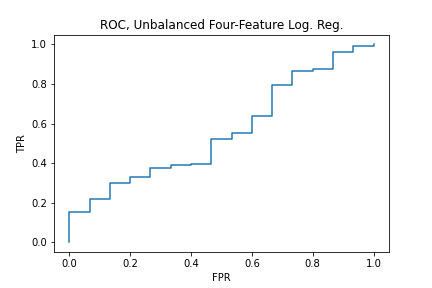
\includegraphics{unbalancedroc}[scale=0.5] 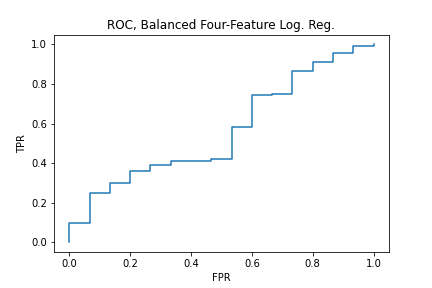
\includegraphics{balancedroc}[scale=0.5]

% \documentclass[10pt,a4paper]{article}
% \usepackage[demo]{graphicx}
% \usepackage{subfig}
% \begin{document}
\begin{figure}[htb]%
    \centering
    {{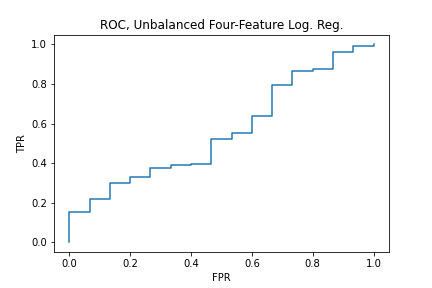
\includegraphics[scale=0.4]{unbalancedroc} }}%
    \qquad
    {{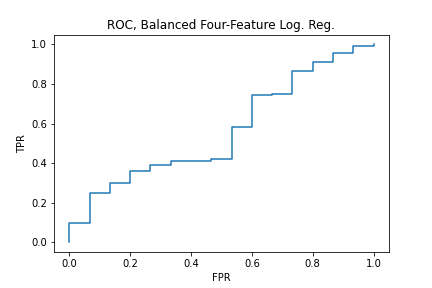
\includegraphics[scale=0.4]{balancedroc} }}%
    % \caption{ROC curves for both four-feature logistic regression models.}%
    \label{fig:example}%
\end{figure}

\subsubsection{Neural Models}

For the four feature input data, we used the largest network that we used on the two feature NN classifier: A $4$ Hidden Layer FC NN, with hidden dimensions of ($1000$, $500$, $500$, $250$) respectively, trained using SGD for $200$ epochs, using weighted cross-entropy Loss. 

With this larger capacity network, we saw an improvement in both train and test accuracy, with a train accuracy of $98.01\%$ and a test accuracy of $95.21\%$.

We hypothesize that this network was able to do perform better than both our two feature model and our non-neural, four feature models because the input data had more features to learn from, and our NN was more expressive, with more learned weights to explain the relationship between our input and targets.

\section{Regression of Admitted White Male Proportions}

In addition to trying to classify using the UC admissions data, we also attempted to do some regression on the data. Specifically, we tried to predict \texttt{AdmMale} using the other $5$ features using a variety of regression techniques.

First, we needed to modify our data in order to use the categorical feature (INS/OOS/INT) in our regressor. We used a one-hot encoding scheme in order to represent this feature. Because our models all have a learned bias term, we drop the INS column in order to avoid rank deficiency in our data matrix. Our transformed data looked like this:

\newline

\begin{tabular}{lrrrrrr}
\toprule
{} &  AppMale &  AdmMale &  AppWhite &  INT &  OOS &  Target \\
Name                        &                    &                    &                     &               &               &                   \\
\midrule
ACALANES HIGH           &           0.450000 &           0.500000 &            0.675000 &             0 &             0 &          0.600000 \\
ADOLFO CAMAR   &           0.553191 &           0.500000 &            0.191489 &             0 &             0 &          0.375000 \\
ADRIAN C WIL    &           0.393939 &           0.285714 &            0.196970 &             0 &             0 &          0.285714 \\
AGOURA HIGH             &           0.542857 &           0.545455 &            0.585714 &             0 &             0 &          0.454545 \\
ALAMEDA SCI &           0.620690 &           0.625000 &            0.206897 &             0 &             0 &          0.375000 \\
\bottomrule
\end{tabular}

We tried 7 different regression models: 
\begin{enumerate}
    \item Ordinary Least Squares (OLS)
    \item Ridge Regression ($L_2$ Regularized Least Squares)
    \item Ridge Regression with Hyperparameter Cross Validation
    \item Lasso ($L_1$ Regularized Least Squares)
    \item Lasso with Hyperparameter Cross Validation
    \item KNeighborsRegressor, a non-parametric regression model
    \item Fully-Connected NN Regressor (same architecture as our 4 Feature FC NN, but trained with an MSE loss)
\end{enumerate}

We got the following MSE on our training and test sets, respectively:

\begin{tabular}{lll}
\toprule
Model &   Training Mean Squared Error &   Testing Mean Squared Error\\
\midrule
OLS & 0.015 & 0.023 \\
Ridge & 0.016 & 0.023 \\
RidgeCV & 0.016 & 0.023 \\
Lasso & 0.041 & 0.040 \\
LassoCV & 0.016 & 0.023 \\
KNeighbors & 0.012 & 0.027 \\
FCNN & 0.012 & 0.022 \\
\bottomrule
\end{tabular}

We see here that our FC NN performed best in terms of minimizing the Mean Squared Error loss in both train and test error. This makes sense, as the FCNN has many degrees of freedom that it can use to represent our data.

\section{Fairness Criterion}

\begin{figure}[htb]%
    \centering
    {{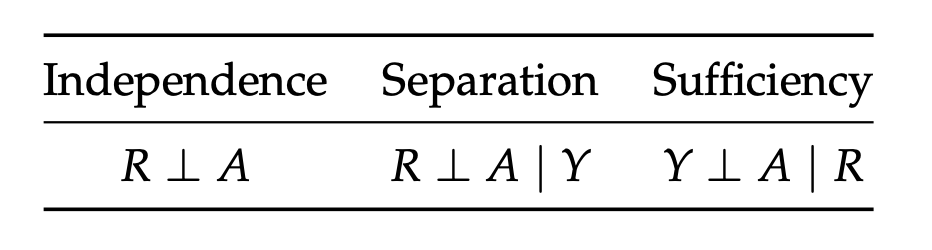
\includegraphics[scale=0.4]{FairnessCriterion} }}%
    \label{fig:example}%
\end{figure}

\subsubsection*{Separation}
\[
P(R=r | Y=y, A=a) \label{eq:separation} \tag{1}
\]
\subsubsection*{Sufficiency}
\[
P(Y=y | R=r, A=a) \label{eq:sufficiency} \tag{2}
\]

In our problem, Y is whether or not a school is in-state (ground truth), R is whether our model predicted a school is in-state (prediction), and A is whether or not a school is predominantly male or predominantly female (sensitive attribute).

We analyzed the predictions made by our 4-feature model to look at the fairness criterions described in "Fairness and machine learning" \cite{barocas-hardt-narayanan}. As described there are three points at which we would want to consider fairness: pre-processing, at training time, and post-processing. Due to the nature of the problem we are analyzing, it was difficult to examine fairness during the first two time frames and so we analyzed the fairness of our model in post-processing.

For both separation and sufficiency we looked at the rate or "probability" for both our model's prediction and the ground truth of whether or not a school was in-state or out-of-state.  

\subsection{Separation and Sufficiency}

\begin{figure}[H]%
    \centering
    {{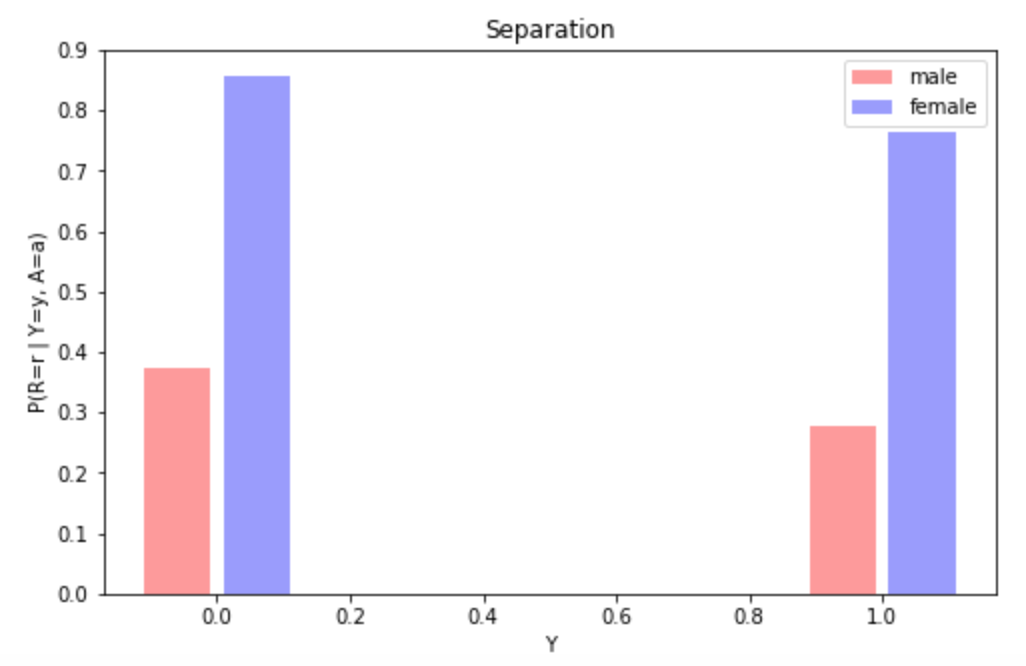
\includegraphics[scale=0.4]{Separation.png} }}%
    {{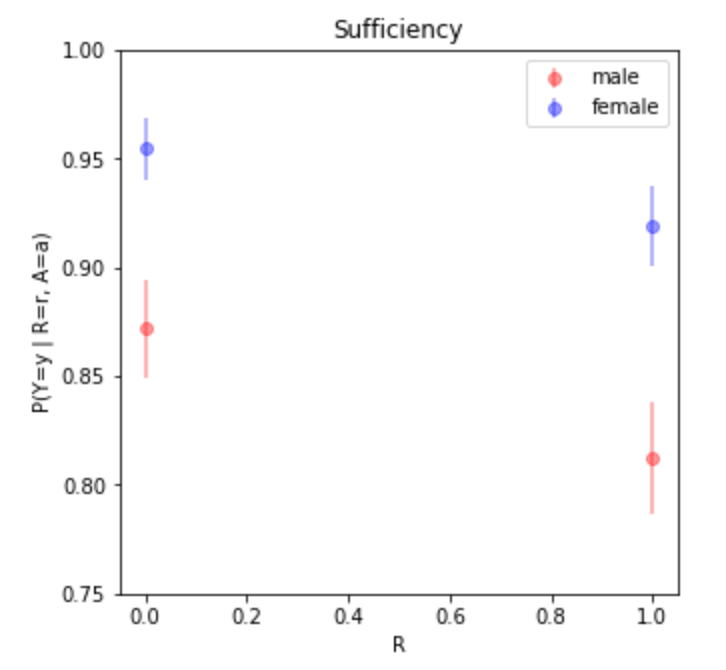
\includegraphics[scale=0.4]{Sufficiency1.png}}}%
    \label{fig:example}%
\end{figure}

We calculated values according to the separation and sufficiency equations above and found that neither were satisfied by our model. With regards to separation, we can see that given the predominant gender of the school's application base, there is a big difference in whether our model predicts the school is in-state (1) vs. out-of-state(0) given the school's true locational status and predominant gender. With regards to sufficiency swe see something very similar in that the ground truth has a wide variation given our model's prediction and the school's predominant gender.

\section{Conclusion}

Despite our extensive analysis of the dataset, we were unable to infer any strong conclusions about the fairness of UC Berkeley admissions process. While the dataset itself is large, its lack of granularity means that even after significant pre-processing, meaningful information is still difficult, if not impossible, to extract. 

Many of the schools we analyzed were missing data necessary for comprehensive analysis, and the inconsistency between data provided by different schools meant that comparing them meaningfully was challenging. If, instead, UC Berkeley released anonymized school district, gender, race, test score, and GPA data per student, omitting districts from which too few students of a certain race/gender applied to ensure anonymity, the data would be significantly more useful. As it stands, this dataset appears to be more of a gesture than a meaningful effort toward transparency in the admissions process.

\printbibliography

\end{document}
